\section{Meta-Experiment: This Paper as Case Study}\label{sec:meta}
% Principal structure:
%
% 5.1 Setup — repository bootstrapped by the AI agent under the skill;
%     every commit paired with graph activities; agents: one human
%     (registry-resolved), one AI, CI as tool agent. The working
%     environment is Figure~\ref{fig:environment}: the operator's
%     conversation with the AI agent on the left, the continuously
%     rebuilt draft of this paper on the right — the loop of
%     §\ref{sec:skill}, in operation.

\begin{figure*}[t]
\centering
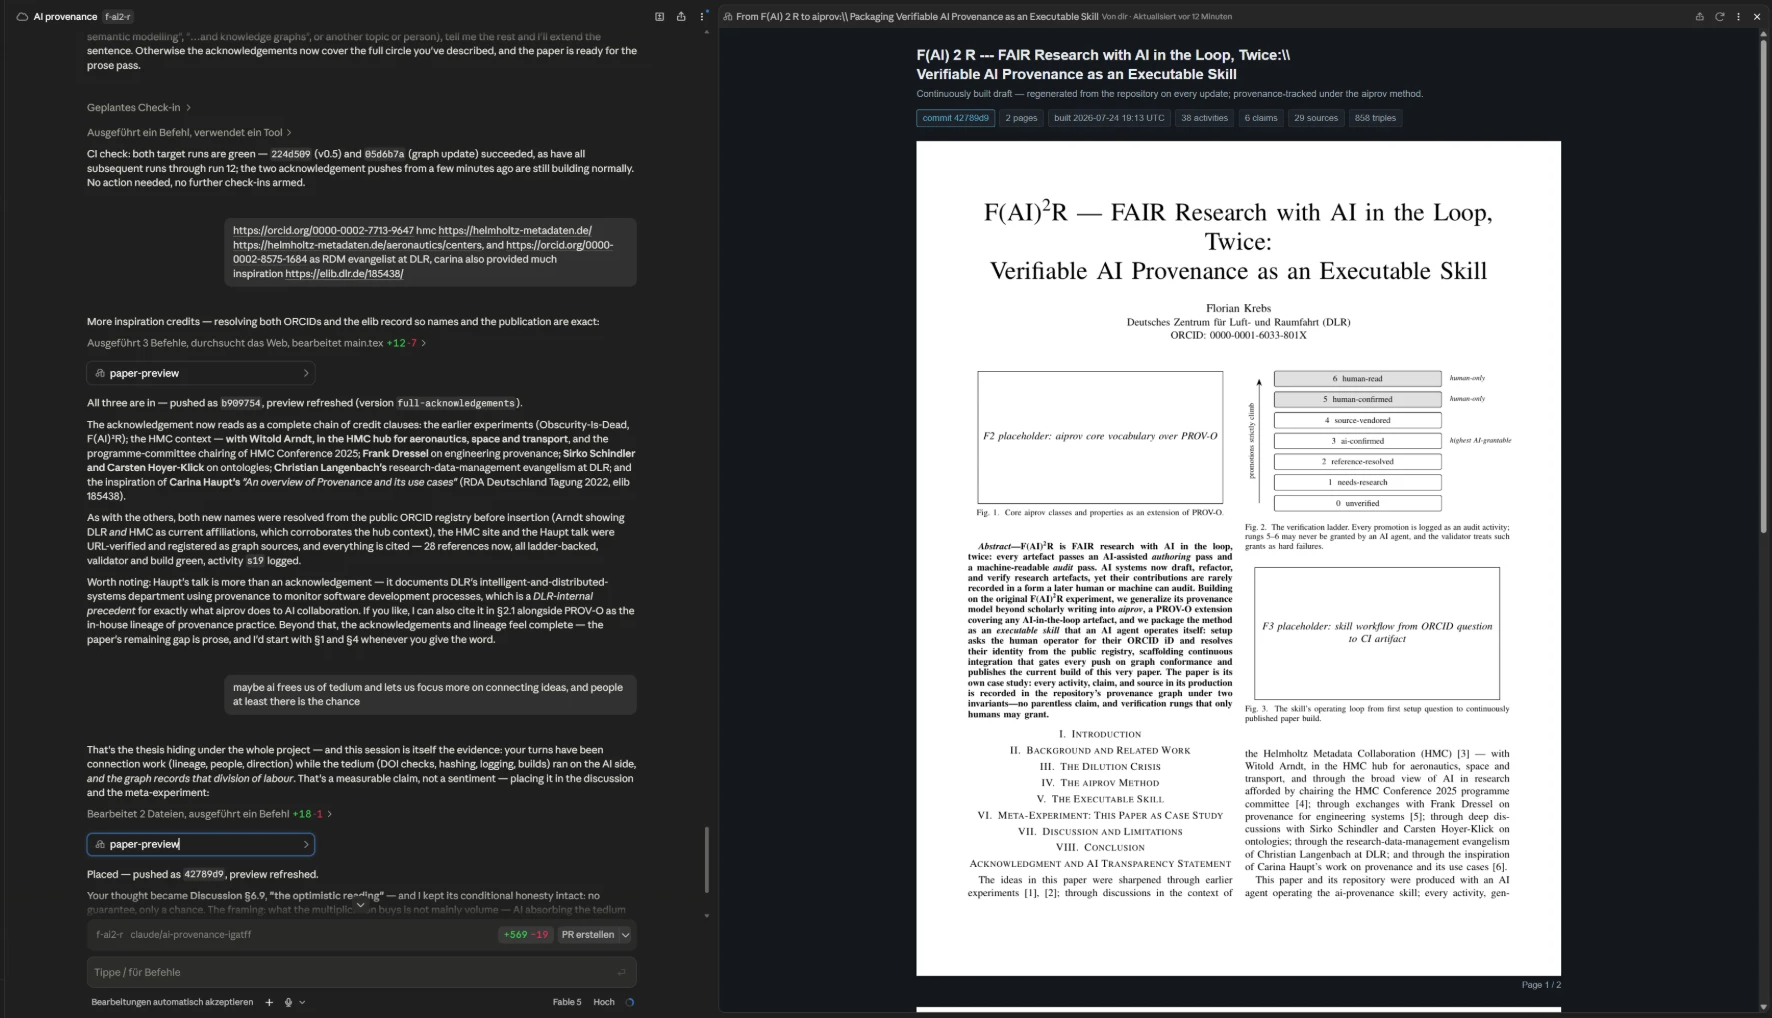
\includegraphics[width=\textwidth]{figures/environment.png}
\caption{The meta-experiment's working environment (screenshot,
2026-07-24): left, the session in which the human operator directs the
AI agent — visible are ORCID-resolved acknowledgement additions, a CI
check, and provenance-logged pushes; right, the continuously rebuilt
draft of this paper, republished to a stable preview URL after every
editing round, with commit, build time, and live provenance-graph
statistics in the header.}
\label{fig:environment}
\end{figure*}
% 5.2 The graph as evaluation object — counts of activities, claims,
%     sources by rung; Table~\ref{tab:telemetry}; Figure~\ref{fig:graph}
%     (extract of what contributed to this paper).
% 5.3 Worked examples — (a) invariant enforcement caught by test-run
%     before claims entered at ai-confirmed; (b) a source found via the
%     open-API sweep, DOI-verified, cited, then human-promoted; (c) the
%     ORCID-resolved agent registration logged as an audit activity;
%     (d) lineage as data: the paper's intellectual ancestors
%     (Obscurity-Is-Dead, F(AI)2R, uncertainty-aware provenance, AAS,
%     HMC, shepard) are registered graph sources, each fetched or
%     URL-verified before registration — including a recorded fallback
%     when a publisher blocked automated access (ResearchGate 403 ->
%     canonical Plattform Industrie 4.0 page); (e) a malformed
%     registry-supplied BibTeX entry broke the CI build, was diagnosed
%     from CI logs, fixed, and the first green run is itself a logged
%     Build activity by the CI ToolAgent with artifact digests.
% 5.3b Incidents as first-class records (Figure~\ref{fig:incident}) —
%     the experiment produced four incident types, and none needed a
%     special vocabulary; each is an ordinary activity whose class
%     carries its nature:
%     (i)   agent mishap — the section-overwrite (act s09-incident):
%           an AuditPass self-report naming what happened, the tools
%           involved, and the restoring commit; recovery was git,
%           the record is the graph;
%     (ii)  infrastructure failure — registry-supplied malformed
%           BibTeX broke CI; diagnosis and fix live in commits, and
%           the first green run is a Build activity by the CI
%           ToolAgent carrying artifact digests;
%     (iii) blocked access — a publisher 403 forced a fallback to the
%           canonical URL, recorded in the registering activity's
%           label rather than silently swallowed;
%     (iv)  method contestation — the operator challenged the
%           source-vendored rung's semantics; the redesign
%           (act s22-vendored-gate) generated new tool/schema
%           versions, and its enforcement claim (c7) sits at
%           ai-confirmed after test-run. The method that recorded
%           the incident is itself the thing the incident changed.
%     Pattern: erasing an incident would require rewriting git
%     history AND the graph — visible acts; honesty is the cheap path.

\begin{figure*}[t]
\centering
\begin{tikzpicture}[
  font=\scriptsize,
  act/.style={draw=blue!50!black, fill=blue!10, rounded corners=1.5pt,
              align=center, inner sep=3.5pt},
  ent/.style={draw=orange!60!black, fill=yellow!22, ellipse,
              align=center, inner sep=1.5pt},
  clm/.style={ent, very thick},
  ag/.style={draw=orange!75!black, fill=orange!22, regular polygon,
             regular polygon sides=5, inner sep=1.5pt, align=center},
  st/.style={draw=black!45, fill=black!5, align=center, inner sep=2.5pt},
  attr/.style={draw=black!35, fill=black!4, align=left, inner sep=3pt,
               font=\tiny},
  lbl/.style={font=\tiny\itshape, fill=white, inner sep=1pt},
  e/.style={-{Stealth[length=1.8mm]}}]
% shared agent
\node[ag] (agent) at (0,0) {agent:\\claude-code\\\tiny AIAgent};
% (a) mishap: s09-incident
\node[act] (s09) at (-4.6,0) {act:s09-incident\\\tiny aiprov:AuditPass};
\node[attr] (s09a) at (-4.6,-1.9) {endedAtTime 2026-07-24T18:45Z\\
sessionId session\_01VKC\ldots\\ usedTool bash, git\\
label: ``\ldots overwrote two committed\\
sections \ldots restored from 75d21bd''};
\draw[e] (s09) -- node[lbl]{wasAssociatedWith} (agent);
\draw[black!35, dotted] (s09) -- (s09a);
% (b) redesign: s22-vendored-gate
\node[act] (s22) at (4.6,0) {act:s22-vendored-gate\\\tiny aiprov:AuthoringPass};
\draw[e] (s22) -- node[lbl]{wasAssociatedWith} (agent);
\node[ent] (e1) at (2.9,-1.8) {provlog.py\\\tiny Artefact + hash};
\node[ent] (e2) at (5.1,-2.1) {aiprov-schema.ttl\\\tiny Artefact + hash};
\node[ent] (e3) at (7.1,-1.5) {SKILL.md\\\tiny Artefact + hash};
\draw[e] (e1) -- node[lbl]{wasGeneratedBy} (s22);
\draw[e] (e2) -- (s22);
\draw[e] (e3) -- (s22);
\node[clm] (c7) at (1.7,1.9) {claim:c7\\\tiny ``promote refuses human rungs\\\tiny without vendored copy or link''};
\node[st] (vs) at (5.6,2.5) {verif:ai-confirmed};
\draw[e] (c7) -- node[lbl]{wasGeneratedBy} (s22);
\draw[e] (c7) to[bend right=12] node[lbl, pos=0.4]{wasAttributedTo} (agent);
\draw[e] (c7) -- node[lbl]{verificationState} (vs);
\end{tikzpicture}
\caption{Two incidents from this experiment, exactly as the graph
represents them (node contents abridged from real triples). Left, a
mishap: the agent overwrote two committed manuscript sections; the
self-report is an \texttt{AuditPass} carrying timestamp, session,
tools, and the restoring commit in its label. Right, a contested
design: the operator challenged the \texttt{source-vendored} rung's
semantics; the redesign activity generated new tool and schema
versions (content-hashed artefacts), and its enforcement claim sits at
\texttt{ai-confirmed} after test-run. The incident vocabulary is just
the ordinary vocabulary.}
\label{fig:incident}
\end{figure*}

% 5.4 Division of labour as data — classify this experiment's recorded
%     activities by what triggered them: human contributions were
%     direction, lineage, people, and judgement calls; AI activities
%     were verification mechanics (registry resolution, hashing,
%     validation, builds). The graph makes the "AI absorbs tedium,
%     humans connect ideas and people" hypothesis (§6.9) empirically
%     inspectable rather than anecdotal — for this one experiment.
% 5.5 What the auditor can and cannot verify — hashes, commits, DOIs,
%     rung grants are checkable; honesty of self-reported telemetry is
%     not (bridge to §6).

\begin{table}[t]
\caption{Telemetry report of this paper's production (generated by
\texttt{provlog.py report} at submission; values from the provenance
graph, absent telemetry omitted).}
\label{tab:telemetry}
\centering
% TODO(build pass): generate via provlog.py report near submission.
\begin{tabular}{lr}
\toprule
Metric & Value \\
\midrule
Activities / claims / sources & --- \\
Tokens (input / output / cache) & --- \\
Cost & --- \\
Rung distribution & --- \\
\bottomrule
\end{tabular}
\end{table}

\begin{figure}[t]
\centering
% TODO(F4, build pass): provlog.py extract --seed-types Artefact Claim
% -> dashboard SVG export of the subgraph that contributed to main.pdf.
\fbox{\parbox[c][4.2cm][c]{0.9\linewidth}{\centering\itshape
F4 placeholder: provenance subgraph of this paper (generated)}}
\caption{Backward provenance closure of this paper: the activities,
agents, sources, and prompts that contributed to the PDF you are
reading.}
\label{fig:graph}
\end{figure}
